% Discription of what is a Artificial Neural Networks and what does it
\chapter{Artificial Neural Networks\authorB} \label{ref:ann}

\section{What is a Artificial Neural Networks?}

  \textbf{A}rtificial \textbf{N}eural \textbf{N}etworks (ANN) are inspired by biological neural networks that constitute animal brains. Important to notice is that they are not faithful models of biologic neural or cognitive phenomena. In fact most of these models are more closely related to mathematical and/or statistical models, for example: clustering algorithms. A clustering algorithm groups a set of objects in such a way that objects in the same group (called a cluster) are more similar (in some sense) to each other than to those in other groups (clusters). Such systems "learn" to perform tasks by considering examples, generally without being programmed with task-specific rules. 
 
\section{Areas of Application}

 ANN are viable computational models for a wide variety of problems, including pattern classification, speech synthesis and recognition, adaptive interfaces between human and complex physical system, function approximation, associative memory, clustering, forecasting and prediction, combinatorial optimization, nonlinear system modeling, and control
 \cite{fundamentals_ann}
 
\section{Components of an ANN}

Simplified an ANN consists of neurons, connection and the weight associated with them, the propagation function, a loss function and a bias. The following sections will give you an introduction what these components represent and how they interact. 

\subsection{Neurons}

Neurons are elementary units in an ANN. A neuron has one ore more inputs and depending on the input values the output value is between 0 and 1. A neuron can get its inputs from other neurons or, if its at the beginning of the network, from an external source. The application determines the structure of the ANN.


\subsection{Connections and weights}

Neurons are connected to neurons in the next layer. It depends on the structure which neurons are connected with which neurons in the next layer. The weights characterize how important a connection between neurons is. 

\begin{figure}[h]
	\centering
	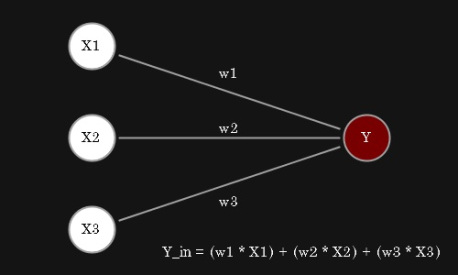
\includegraphics[width=0.7\textwidth]{./media/images/weights1.jpg}
  	\caption{Simple Picture to explain  Weights
  	\\Source: https://tinyurl.com/smw9bk4}
  	\label{Gvon}
\end{figure}

\textbf{For example:}\newline
A neuron, we call it Y for this example, has three neurons connected to it as inputs. These neurons are called X1, X2 and X3. The weight of the connection of X1 has a bigger weight than the connections X2 and X3. That means the output of Y depends more on the input of X1 because the input from Y is made up from the three input neurons times their weights summed up.

\subsection{Propagation function, activation function and Bias}

The propagation function takes the input values of a neuron, the weight of each connections and the bias and adds them up. The resulting value is processed by the activation function which sets the output. One of the most common activation function is the sigmoid function, because it is not a step function which means the output does not  change instantaneously. That is important for the training algorithm because with that the output of a neuron can not only be 1 or 0. It can be any number between 1 and 0 and it gives an answer for how certain it is. Therefore the training will be easier because it is easier to find out in which directions and how much the weights should be changed. The bias is a neuron which has no inputs. A bias is used to shift the decision boundary to the left or right.

\section{Organization}

A artificial neural network can be organized in many different ways.

\subsection{Feed Forward ANN}

\begin{figure}[h]
	\centering
	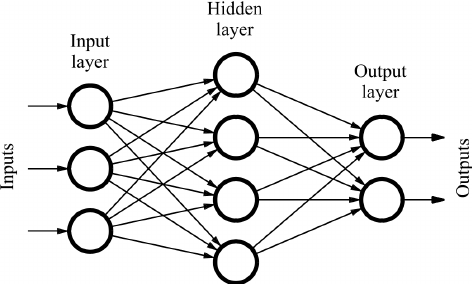
\includegraphics[width=0.7\textwidth]{./media/images/feed_forward_neural_network.png}
  	\caption{Feed forward network
  	\\Source: https://tinyurl.com/ydzdtqqx}
  	\label{ffNN}
\end{figure}

Fig. 3.2 demonstrates a feed forward ANN .There are a variable number of hidden layers depending on the purpose of the neural network. Nothing in the hidden layer is visible. 

\subsection{CNN}

Convolution Neural Network (CNN) is the most important network organization for this task. It is based on the human visual cortex and is optimal for image and video recognition. The components of a CNN are a series of convolution and sub-sampling layers followed by a fully connected layer and a normalizing layer.

How a CNN works will be explained in the following example. The same example like in "Review of Deep Learning Algorithms and Architectures"\cite{exampleCNN} will be used
\begin{figure}[h]
	\centering
	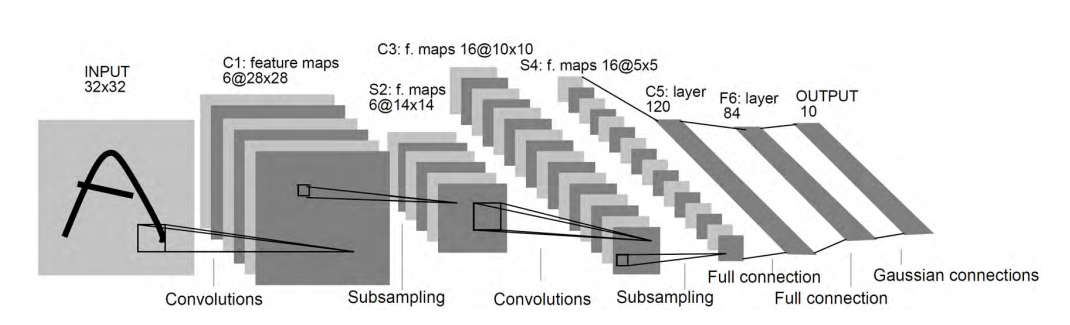
\includegraphics[width=1.1\textwidth]{./media/images/CNN.PNG}
  	\caption{7-layer architecture of CNN for character recognition
  	\\ \cite[Fig.~4.]{exampleCNN}}
  	\label{CNN}
\end{figure}

Progressively more refined feature extraction at every layer is performed by the series of multiple convolution layers. This process is moving from input to output layer. After the convolution layers there are fully connected layers that perform classification. There is also the possibility of putting Sub-sampling or pooling layers between each convolution layer. The input of a CNN is a 2D n*n pixelated image. Each layer consists of filters or kernels (groups of 2D neurons). In most neural networks neurons in each feature extraction layer are connected to all neurons in the adjacent layers. But in a CNN they are only connected to the spatially mapped fixed sized and partially overlapping neurons in the previous layer’s input image or feature map.

\section{Encoder-Decoder-Based Architecture}

Encoder-Decoder-Based networks are networks, which try to reconstruct their own input. You construct the network so that it reduces the input size by using one or more hidden layers, until it reaches a reasonably small hidden layer in the middle. As a result your data has been compressed (encoded) into a few variables. From this hidden representation the network tries to reconstruct (decode) the input again.

In order to do a good job at reconstructing the input the network has to learn a good representation of the data in the middle hidden layer. This can be useful for dimensionality reduction, or for generating new “synthetic” data from a given hidden representation. This is especially important considering that we are trying to construct a 3D map out of the camera input. 









